\chapter{Dasar Teori}
\label{chap:dasar_teori}
Pada bab ini akan dijelaskan dasar-dasar teori mengenai Android SDK, Google VR SDK,Quaternion, \textit{Sensor Fusion}, dan algoritma \textit{Head Motion Detection}.

% 2.1 Android SDK
\section{Android SDK}
\label{sec:android_sdk}

Android SDK(\textit{software development kit}) adalah kumpulan \textit{source code, development tools, emulator,}\cite{developers2011android} dan semua \textit{libraries} untuk membuat suatu aplikasi untuk \textit{platform} Android. IDE (\textit{integrated development environment} yang resmi untuk Android SDK adalah Android Studio. Android Studio dapat di download di halaman situs web Google Developer\cite{developers2011android}, sekaligus dengan Android SDKnya.  

% 2.1.1 Struktur File Android Studio Project
\subsection{Struktur File Android Studio Project}
Pada saat \textbf{project} baru telah dibuat, Android Studio akan membuatkan folder-folder standar (Gambar \ref{fig:android-studio-structure}). Berikut adalah sebagian penjelasan dari hal yang perlu di perhatikan pada struktur tersebut:
\begin{itemize}
	\item Folder \textbf{\textit{module}/build} mengandung file-file dari hasil pembangunan \textit{project}.
	\item Folder \textbf{\textit{module}/libs} mengandung \textit{libraries} privat.
	\item Folder \textbf{\textit{module}/src} mengandung semua kode dan file sumber untuk suatu modul yang terbagi menjadi \textit{subdirectories} berikut:
	\begin{itemize}
		\item Folder \textbf{androidTest/} mengandung kode untuk mengetes yang berjalan di perangkat Android. 
		\item Folder \textbf{main/} mengandung file-file kode dan file sumber inti dari suatu module yang terbagi menjadi \textit{subdirectories} berikut:
		\begin{itemize}
			\item File \textbf{AndroidManifest.xml} mendeskripsikan sifat dari aplikasi dan setiap komponennya. 
			\item Folder \textbf{java/} mengandung kode java.
			\item Folder \textbf{jni/} mengandung kode yang menggunakan Java Native Interface (JNI).
			\item Folder \textbf{gen/} mengandung file java yang dihasilkan oleh Android Studio.
			\item Folder \textbf{res/} mengandung file-file sumber untuk aplikasi, seperti file drawable, layout, dan UI String.
			\item Folder \textbf{assets/} mengandung file yang akan di kompile menjadi file \textbf{.apk}. File-file yang biasa disimpan di folder ini adalah file audio, video, file html, gambar dan file bantu lainnya.
		\end{itemize}
		\item File \textbf{build.gradle}(module) mendefinisikan konfigurasi modul untuk proses \textit{build}.
	\end{itemize}
	\item File \textbf{build.gradle}(project) mendefinisikan konfigurasi proses \textbf{build} untuk \textit{project} yang berlaku untuk semua modul.
\end{itemize}
Folder \textbf{App} pada Gambar \ref{fig:android-studio-structure} merupakan folder \textit{module}.
\begin{figure}[htbp]
	\centering
		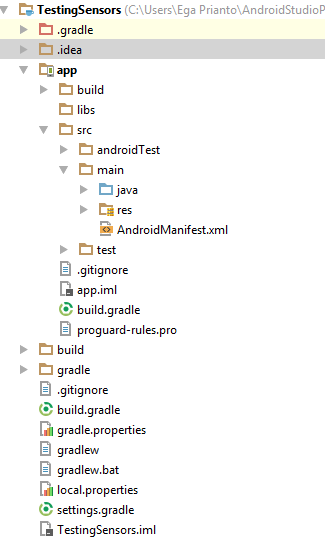
\includegraphics[scale=1]{Gambar/android-studio-structure.png}
	\caption{Tampilan struktur folder pada \textit{project} Android Studio}
	\label{fig:android-studio-structure}
\end{figure}

% 2.1.2 Membuat User Interface
\subsection{Membuat User Interface}
Pada subbab ini akan dijelaskan bagaimana membuat layout di XML termasuk \textit{text field} dan \textit{button}

% Sub 2.1.2 Hierarki (GUI) untuk Aplikasi Android
\subsubsection{Hierarki \textit{Graphical User Interface} (GUI) untuk Aplikasi Android}
GUI untuk aplikasi Android dibuat dengan hierarki dari objek View dan ViewGroup (Gambar \ref{fig:viewgroup}). Objek-objek dari View biasanya adalah \textit{UI(User Interface) Widgets} seperti \textit{button} atau \textit{text field}. Objek-objek dari ViewGroup tidak terlihat oleh \textit{view containers} yang mendefinisikan bagaimana \textit{child views} ditata seperti \textit{grid} atau \textit{vertical list}.

\begin{figure}[htbp]
	\centering
		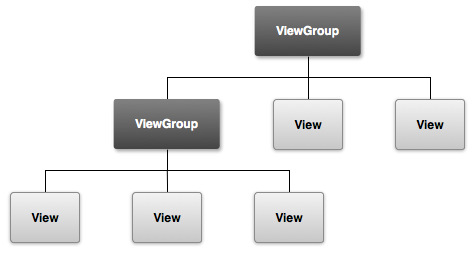
\includegraphics[scale=1]{Gambar/viewgroup.png}
	\caption{Illustrasi bagaimana percabangan objek ViewGroup pada \textit{layout} dan mengandung objek View lainnya.}
	\label{fig:viewgroup}
\end{figure}

Android menggunakan file XML yang berkorespondesi kepada \textit{subclasses} dari View dan ViewGroup, sehingga UI dapat didefinisikan dalam XML menggunakan hierarki dari elemen UI.

\subsubsection{Attribut-attribut Objek View}
Pada subbab ini akan dijelaskan attribut-attribut object View yang digunakan dalam membuat GUI pada file activity\_main.xml
\begin{itemize}
	\item \textbf{android:id}
	Attribut ini merupakan pengidentifikasi dari suatu view. Attribut ini dapat digunakan untuk menjadi referrensi object dari kode aplikasi seperti membaca dan memanipulasi objek tersebut (Akan dijelaskan lebih lanjut pada subbab \ref{sec:activity}). Tanda '@' dibutuhkan ketika mereferensi object dari suatu XML. Tanda '@' tersebut diikuti dengan tipe (id pada kasus ini), \textit{slash}, dan nama (edit\_message pada kode \ref{lst:attribute-view}). Tanda tambah (+) sebelum tipe hanya dibutuhkan jika ingin mendefinisikan \textit{resource ID} untuk pertama kalinya.
	\item \textbf{android:layout\_width} dan \textbf{android:layout\_height}
	Attribut ini digunakan untuk mendefinisikan panjang dan lebar dari suatu objek View. Daripada menggunakan besar spesifik untuk panjang dan lebarnya, lebih baik menggunakan "wrap\_content" yang menspesifikasi viewnya hanya akan sebesar yang dibutuhkan untuk memuat konten-konten dari View. Jika menggunakan "match\_parent" pada kasus kode \ref{lst:attribute-view} View akan memenuhi layar, karena besarnya akan mengikuti besar dari paretnya LinearLayout.


	\item \textbf{android:hint}
	Attribut ini merupakan \textit{default string} untuk di tampilkan ketika objek View kosong. Daripada menggunakan \textit{hard-coded string} sebagai \textit{nilai} untuk ditampilkan, \textit{value} "@string/edit\_message" mereferensi ke sumber string pada file yang berbeda. Karena mereferensi ke sumber konkrit, maka tidak dibutuhkan tanda tambah (+). Nilai string ini akan di simpan pada file Strings.xml yang ditunjukkan pada Kode \ref{lst:string-xml}.
	\begin{lstlisting}[caption={Contoh kode pada string.xml},label={lst:string-xml},language=xml]
	<resources>
    <string name="app_name">MyFirstAndroidApp</string>
    <string name="edit_message">Ini adalah hint</string>
    <string name="button_send">Send</string>
	</resources>

\end{lstlisting}


	\item \textbf{android:onClick}
	Attribut ini akan memberitahu \textit{system} untuk memanggil method yang sesuai namanya (contoh pada kode \ref{lst:attribute-view} adalah \textbf{sendMessage()}) di Activity ketika pengguna melakukan klik pada \textit{button} tersebut. Agar \textit{system} dapat memanggil method yang tepat, method tersebut harus memenuhi kriteria berikut.
	\begin{itemize}
		\item \textit{Access Modifier} haruslah \textit{public}.
		\item Harus \textit{void return value}nya.
		\item Mempunyai View sebagai parameter satu-satunya. View ini akan diisi dengan View yang di klik.
	\end{itemize}
\begin{lstlisting}[caption={Contoh kode file XML pada folder layout},label={lst:attribute-view},language=xml]
	<LinearLayout
		xmlns:android="http://schemas.android.com/apk/res/android"
		xmlns:tools="http://schemas.android.com/tools"
		android:layout_width="match_parent"
		android:layout_height="match_parent"
		android:orientation="horizontal">
		<EditText android:id="@+id/edit_message"
				android:layout_weight="1"
				android:layout_width="0dp"
				android:layout_height="wrap_content"
				android:hint="@string/edit_message" />
		<Button
				android:layout_width="wrap_content"
				android:layout_height="wrap_content"
				android:text="@string/button_send"
				android:onClick="sendMessage" />
	</LinearLayout>
\end{lstlisting}
\end{itemize}


\subsection{Activity}
\label{sec:activity}
Activity adalah suatu hal yang terfokuskan dengan apa yang bisa pengguna lakukan. Hampir semua \textit{Activity} berinteraksi dengan pengguna, jadi kelas Activity akan membuat suatu halaman baru yang bisa ditambahkan dengan konten-konten View. Selain Activity dapat direpresentasikan kepada pengguna dengan halaman \textit{full-screen}, Activity juga dapat direpresentasikan dengan cara lain: seperti halaman \textit{floating} atau tertanam di Activity lain.

\subsubsection{Activity Lifecycle}

\begin{figure}[htbp]
	\centering
		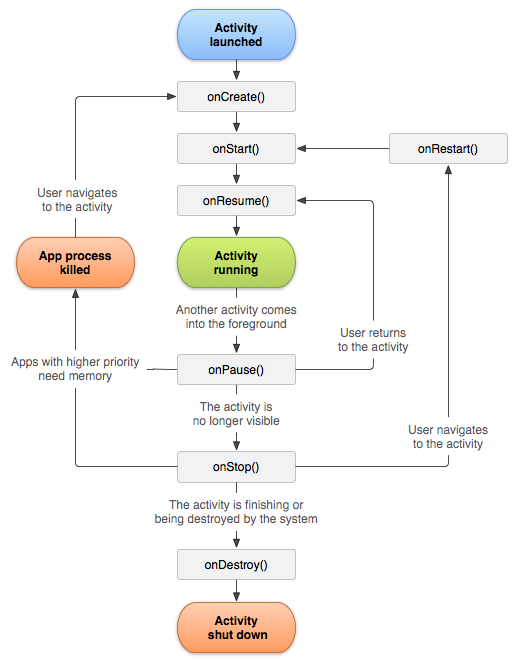
\includegraphics[scale=0.48]{Gambar/activity-lifecycle.png}
	\caption{\textit{State diagram} siklus Activity}
	\label{fig:activity-lifecycle}
\end{figure}

Aktivitas dalam sistem android di atur sebagai \textit{activity stack}. Ketika ada Activity baru yang dimulai, Activity tersebut ditempatkan di paling atas pada \textit{stack} dan menjadi Activity aktif. Activity sebelumnya akan tetap berada di bawah stack, dan tidak akan muncul lagi sampai Activity yang baru berakhir. 

Activity didasari dari empat kondisi:
\begin{itemize}
	\item Jika Activity berada di latar depan pada layar, Activity tersebut sedang aktif.
	\item Jika Activity sudah tidak terfokuskan tetapi masih dapat terlihat, Activity tersebut sedang berhenti sementara. Pada kondisi ini Activity tersebut masih berjalan, tapi bisa diberhentikan ketika system berada dalam situasi kekurangan memori.
	\item Jika suatu Activity benar-benar dihalangi oleh Activity lain, Activity tersebut telah berhenti. Activity tersebut akan tetap mengingat seluruh keadaan dan infomasi anggota tetapi, Activity tersebut tidak lagi terlihat oleh pengguna jadi tampilan jendelanya akan tersembunyi dan seringkali akan diberhentikan Activitynya ketika system membutuhkan memori.
	\item Jika suatu Activity sedang berhenti sementara atau berhenti total, sistem dapat membuang Activity dari memory dengan cara menanyakan kepada pengguna untuk memberhentikannya atau langsung diberhentikan oleh sistem. Jika Activity tersebut ditampilkan lagi kepada pengguna, Activity tersebut harus memulai dari awal dan kembali ke keadaan sebelumnya.
\end{itemize}
Gambar \ref{fig:activity-lifecycle} menunjukkan pentingnya alur keadaan dari suatu Activity. Gambar segi empat merepresentasikan \textit{callback methods} yang dapat diimplementasikan untuk melakukan operasi ketika Activity berubah kondisi. Oval berwarna merupakan kondisi-kondisi utama dari suatu Activity.
Ada 3 \textit{key loops} untuk memantau suatu Activity:
\begin{itemize}
	\item \textit{Entire lifetime} terjadi diantara pemanggilan pertama pada onCreate(Bundle) sampai ke satu pemanggilan akhir onDestroy(). Suatu Activity akan melakukan semua persiapan pada kondisi umum pada method onCreate(), dan melepaskan seluruh sisa pemrosesan pada method onDestroy().
	\item \textit{Visible lifetime} terjadi antara pemanggilan onStart() sampai pemanggilan yang sesuai pada onStop(). Pada tahap ini pengguna dapat melihat Activity pada layar meskipun tidak berada pada \textit{foreground} dan berinteraksi dengan pengguna.
	\item \textit{Foreground lifetime} terjadi antara pemanggilan method onResume() sampai ke satu pemanggilan akhir onDestroy(). Pada tahap ini Activity berada di depan semua Activity lainnya dan sedang berinteraksi dengan user.
\end{itemize}


\subsection{Android Sensor Framework}
\label{sec:android_sensor_framework}
Sebagian besar dari perangkat android sudah memiliki sensor yang mengukur gerakan, orientasi, dan berbagai keadaan lingkungan. Sensor-sensor ini dapat memberikan data mentah dengan tingkat akurasi yang tinggi. Sensor ini juga berguna untuk memantau pergerakan tiga dimensi atau posisi perangkat. Sensor ini juga dapat memantau perubahan keadaan lingkungan yang dekat dengan perangkat. 
Android mendukung tiga kategori sensor:
\begin{itemize}
	\item \textbf{Sensor gerak}
	Sensor-sensor ini mengukur akselerasi dan rotasi pada tiga sumbu. Kategori sensor ini meliputi \textit{accelerometers}, sensor gravitasi, \textit{gyroscope}, dan rotasi vektor. 
	\item \textbf{Sensor keadaan lingkungan}
	Sensor-sensor ini mengukur berbagai keadaan lingkungan seperti suhu udara, tekanan, pencahayaan, dan kelembaban. Kateori sensor ini termasuk barimeter, fotometer dan termometer.
	\item \textbf{Sensor posisi}
	Sensor-sensor ini mengukur posisi perangkat. Kategori sensor ini meliputi sensor orientasi dan magnetometer.
\end{itemize}
Android Sensor Framework membantu developers untuk mengakses berbagai jenis sensor. Beberapa sensor berbasis perangkat keras dan beberapa sensor berbasis perangkat lunak. Sensor berbasis perangkat keras mendapatkan data dengan langsung mengukur sifat lingkungan tertentu, seperti percepatan, kekuatan medan geomagnetik, atau perubahan sudut. Sensor berbasis perangkat lunak mendapatkan data dari satu atau lebih sensor berbasis perangkat keras. Sensor berbasis perangkat lunak ini juga terkadang disebut sensor virtual atau sensor sintetis. Pada tabel berikut akan dirincikan tipe-tipe setiap sensor posisi dan gerak, deskripsi, dan penggunaan umumnya.

\begin{table}[htbp]
	\centering
	\caption{Tipe-tipe Sensor pada Android}
\begin{tabular}{|p{6.3cm}| p{1.5cm}| p{5cm}| p{2.4cm}|} 
\hline
Sensor & Tipe & Deskripsi & Penggunaan umum\\ \hline
TYPE\_ACCELEROMETER & Perangkat Keras & Mengukur percepatan dalam \(m/s^2\) yang terjadi pada perangkat di semua tiga sumbu fisik (x,y,z), termasuk percepatan gravitasi. & Deteksi gerak(goncangan, keseimbangan, dan lain-lain)\\ \hline
TYPE\_GRAVITY & Perangkat Lunak atau Perangkat Keras & Mengukur percepatan gravitasi dalam \(m/s^2\) yang terjadi pada perangkat di tiga sumbu fisik (x,y, dan z) & Deteksi gerak(goncangan, keseimbangan, dan lain-lain)\\ \hline
TYPE\_GYROSCOPE & Perangkat Keras & Mengukur rata-rata rotasi sudut dalam \(rad/s\) di tiga sumbu fisik (x,y, dan z). & Deteksi rotasi (putaran, belokan, dan lain-lain).\\ \hline
TYPE\_LINEAR\_ACCELERATION & Perangkat Lunak atau Perangkat Keras & Mengukur percepatan dalam \(m/s^2\) yang terjadi pada perangkat di semua tiga sumbu fisik (x,y,z), tidak termasuk percepatan gravitasi. & Memantau percepatan pada suatu sumbu.\\ \hline
TYPE\_MAGNETIC\_FIELD & Perangkat Keras & Mengukur medan magnet sekitar untuk semua tiga sumbu fisik (x,y, dan z) di satuan \(\mu T\). & Membuat Kompas.\\ \hline
TYPE\_ORIENTATION & Perangkat Lunak & Mengukur derajat rotasi yang terjadi pada perangkat pada semua tiga sumbu fisik (x,y, dan z). & Menentukan posisi perangkat \\ \hline
TYPE\_ROTATION\_VECTOR & Perangkat Lunak dan Perangkat Keras & Mengukur orisentasi dari suatu perangkat dengan menyediakan tiga element dari vektor rotasi perangkat. & Deteksi gerak dan deteksi rotasi.\\ \hline
\end{tabular}
\end{table}
\subsubsection{Sistem Koordinat Sensor}
\label{sec:sistem_koordinat_sensor}
Pada umumnya, sensor framework menggunakan sistem tiga sumbu koordinat standar untuk mengekspresikan nilai data. Sebagian besar sensor sistem koordinat didefinisikan relatif terhadap layar perangkat bila perangkat dibuat dalam orientasi standar (lihat Gambar \ref{fig:axis-device})
\begin{figure}[htbp]
	\centering
		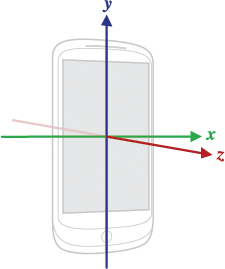
\includegraphics[scale=1]{Gambar/axis-device.png}
	\caption{Sistem koordinat (relatif dengan perangkatnya) yang digunakan oleh Sensor API}
	\label{fig:axis-device}
\end{figure}
Sensor-sensor yang menggunakan sistem tiga sumbu seperti Gambar \ref{fig:axis-device} adalah sebagai berikut :
\begin{itemize}
	\item Accelerometer
	\item Sensor Gravitasi
	\item Gyroscope
	\item Sensor Percepatan Linear
	\item Sensor Medan Geomagnetik
\end{itemize}
Koordinat sistem yang sumbunya tidak tertukar ketika orientasi perangkat berubah. Sistem koordinat sensor tidak pernah berubah seiring perangkatnya bergerak. Dalam aplikasi android tidak dapat diassumsikan bahwa standar orientasi perangkat android adalah \textit{portrait}. Kebanyakan perangkat \textit{Tablet} standar orientasinya adalah \textit{landscape}. Sistem koordinat sensor selalu di dasarkan pada orientasi dasar dari suatu perangkat android.
\subsubsection{Struktur Nilai yang Dikembalikan oleh Sensor}
Nilai dari sensor akan didapatkan ketika ada perubahan nilai pada sensor. Setiap sensor memiliki ketelitian perubahan nilai yang berbeda-beda. Nilai ini akan didapatkan dengan tipe data array of float. Besar dan isi dari array tergantung pada sensor yang sedang di pantau.\\
\textbf{TYPE\_ACCELEROMETER}\\
Semua nilai didefinisikan sebagai satuan \(m/s^2\)
\begin{itemize}
	\item values[0]: Percepatan yang terjadi pada sumbu x dikali -1
	\item values[1]: Percepatan yang terjadi pada sumbu y dikali -1
	\item values[2]: Percepatan yang terjadi pada sumbu z dikali -1
\end{itemize}
Sensor ini mengukur percepatan(\(Ad\)) yang diterapkan pada perangkat. Sensor tersebut dapat mengukur percepatan dengan mengukur gaya(\(Fs\)) yang terjadi pada sensor menggunakan relasi berikut:
\[
	Ad = -\Sigma Fs / mass
\]
Secara khusus, gravitasi selalu mempengaruhi percepatan yang diukur :
\[
	Ad =  -g -\Sigma F / mass
\]
Karena inilah ketika perangkat android sedang diam, accelerometer membaca percepatan gravitasi sebesar \(g = 9.81m/s^2\).
Demikian pula ketika perangkat android sedang dalam keadaan jatuh bebas. Perangkat akan mempercepat menuju ke tanah pada percepatan \(9.81 m/s^2\), sehingga accelerometer membaca percepatan total sebesar \( 0 m/s^2\). 
Suatu saat akan di butuhkan untuk mengukur percepatan asli yang terjadi pada perangkat, sehingga kontribusi gravitasi harus di eliminasi. Hal ini bisa dilakukan dengan menerapkan \textit{high-pass} filter. Sebaliknya, \textit{low-pass} filter dapat digunakan untuk mendapatkan nilai gravitasi saja. 
\begin{lstlisting}[caption={Implementasi \textit{low-pass} filter},label={lst:low-pass-filter},language=java]
	 public void onSensorChanged(SensorEvent event)
     {
          // alpha dikalkulasikan sebagai t / (t + dT)
          // dengan t adalah low-pass filter's time-constant
          // dan dT, rata-rata event tersampaikan

          final float alpha = 0.8;

          gravity[0] = alpha * gravity[0] + (1 - alpha) * event.values[0];
          gravity[1] = alpha * gravity[1] + (1 - alpha) * event.values[1];
          gravity[2] = alpha * gravity[2] + (1 - alpha) * event.values[2];

          linear_acceleration[0] = event.values[0] - gravity[0];
          linear_acceleration[1] = event.values[1] - gravity[1];
          linear_acceleration[2] = event.values[2] - gravity[2];
     }
\end{lstlisting}
\textit{Low-pass} filter dapat diimplementasikan pada kode \ref{lst:low-pass-filter}\\
\textbf{TYPE\_MAGNETIC\_FIELD}\\
Sensor ini mengukur medan magnet sekitar perangkat pada sumbu X,Y, dan Z dalam satuan micro-Tesla.\\
\textbf{TYPE\_GYROSCOPE}\\
Sensor ini mengukur rata-rata perputaran pada perangkat yang berputar di sumbu X,Y, dan Z dalam satuan radians/second. Sistem koordinat yang digunakan sama dengan sistem koordinat pada sensor percepatan(Accelerometer). Jika perangkat berputar berlawanan arah jarum jam pada sumbu tertentu, maka rotasi yang terjadi akan bernilai positif. Perhatikan bahwa standar perputaran ini adalah definisi matematika standar pada rotasi positif.
\begin{itemize}
	\item values[0]: Percepatan angular pada sumbu X.
	\item values[1]: Percepatan angular pada sumbu Y.
	\item values[2]: Percepatan angular pada sumbu Z.
\end{itemize}
Biasanya keluaran dari gyroscope terintegrasi dari waktu ke waktu untuk menghitung rotasi yang menggambarkan perubahan sudut atas langkah waktu, misalnya pada kode \ref{lst:gryoscope-example}
\begin{lstlisting}[caption=contoh implementasi gyroscope,label={lst:gryoscope-example},language=java]
	  private static final float NS2S = 1.0f / 1000000000.0f;
     private final float[] deltaRotationVector = new float[4]();
     private float timestamp;

     public void onSensorChanged(SensorEvent event) {
          // Pada tahapan ini delta rotasi akan dikalikan dengan rotasi saat ini
          // setelah mengomputasinya dari data gyro.
          if (timestamp != 0) {
              final float dT = (event.timestamp - timestamp) * NS2S;
              // Sumbu dari rotasi, masih belum di normalisasi.
              float axisX = event.values[0];
              float axisY = event.values[1];
              float axisZ = event.values[2];

              // Menghitung percepatan angular
              float omegaMagnitude = sqrt(axisX*axisX + axisY*axisY + axisZ*axisZ);

              // Normalisasi rotasi vektor jika cukup besar untuk mendapatkan sumbunya.
              if (omegaMagnitude > EPSILON) {
                  axisX /= omegaMagnitude;
                  axisY /= omegaMagnitude;
                  axisZ /= omegaMagnitude;
              }

              // Integrate around this axis with the angular speed by the time step
              // in order to get a delta rotation from this sample over the time step
              // We will convert this axis-angle representation of the delta rotation
              // into a quaternion before turning it into the rotation matrix.
              float thetaOverTwo = omegaMagnitude * dT / 2.0f;
              float sinThetaOverTwo = sin(thetaOverTwo);
              float cosThetaOverTwo = cos(thetaOverTwo);
              deltaRotationVector[0] = sinThetaOverTwo * axisX;
              deltaRotationVector[1] = sinThetaOverTwo * axisY;
              deltaRotationVector[2] = sinThetaOverTwo * axisZ;
              deltaRotationVector[3] = cosThetaOverTwo;
          }
          timestamp = event.timestamp;
          float[] deltaRotationMatrix = new float[9];
          SensorManager.getRotationMatrixFromVector(deltaRotationMatrix, deltaRotationVector);
          // User code should concatenate the delta rotation we computed with the current rotation
          // in order to get the updated rotation.
          // rotationCurrent = rotationCurrent * deltaRotationMatrix;
     }
     }
\end{lstlisting}
Dalam prakteknya, gyroscope \textit{noise} dan \textit{offset} akan menyebabkan beberapa kesalahan yang harus dikompensasi. Cara untuk mengkompensasinya biasanya dilakukan dengan menggunakan informasi dari sensor lain.\\
\textbf{TYPE\_GRAVITY}\\
Sensor ini menunjukkan arah dan besarnya vektor gaya gravitasi. Sensor ini mengembalikan nilai dengan satuan \(m/s^2\). Sistem koordinat sama seperti sistem koordinat yang umum digunakan sensor percepatan. 

Catatan: Bila perangkat sedang diam, maka keluaran dari sensor gravitasi harus identik dengan accelerometer. \\
\textbf{TYPE\_LINEAR\_ACCELERATION}\\
Sensor yang menunjukkan percepatan pada setiap sumbu perangkat, tidak termasuk percepatan yang terjadi karena gravitasi. Nilai diberikan dalam satuan \(m/s^2\). Sistem koordinat yang digunakan sama seperti sistem koordinat yang digunakan sensor percepatan. Keluaran dari sensor accelerometer, gravitasi dan percepatan linear harus mengikuti aturan berikut:
\[
	percepatan = gravitasi + percepatan linear
\]\\
\textbf{TYPE\_ORIENTATION}\\
Semua nilai adalah sudut dalam derajat.
\begin{itemize}
	\item values[0]: Azimuth, sudut diantara arah magnetik utara dengan sumbu y, sekitar sumbu z (0 sampai 359). 0 = Utara, 90 = Timur, 180 = Selatan, 270 = Barat
	\item values[1]: Pitch, rotasi sekitar sumbu x (-180 sampai 180), dengan nilai positif ketika sumbu x bergerak menuju sumbu y.
	\item values[2]: Roll, perputaran sekitar sumbu y (-90 sampai 90) pada kondisi potrait, sensor akan bernilai 0. Pada kondisi landscape ke kanan sensor akan bernilai 90 dan sebaliknya yaitu kondisi landscape ke kiri sensor akan bernilai -90.
\end{itemize}

Catatan: Definisi ini berbeda dengan definisi yaw, pitch, dan roll yang digunakan pada aviasi yang sumbu X adalah sepanjang sisi bidang.

Catatan: Sensor ini sudah tidak digunakan lagi(deprecated), yang digunakan sekarang adalah sensor rotasi vector.\\
\textbf{TYPE\_ROTATION\_VECTOR}\\
Sensor ini merepresentasikan orientasi perangkat dengan kombinasi dari sumbu dan sudut. Perangkat akan di putar sebesar sudut \(\theta\) mengelilingi sumbu \(x,y,z\). Tiga elemen dari vektor rotasi adalah (\(x \sin (\frac{\theta}{2}), y \sin (\frac{\theta}{2}), z \sin (\frac{\theta}{2})\)), sehingga besarnya vektor rotasi sama dengan \(\sin (\frac{\theta}{2})\), dan arah vektor rotasi sama dengan sumbu rotasi. Tiga elemen dari vektor rotasi sama dengan tiga komponen terakhir pada unit quaternion(\(\cos (\frac{\theta}{2}),x \sin (\frac{\theta}{2}), y \sin (\frac{\theta}{2}), z \sin (\frac{\theta}{2})\)) yang dijelaskan pada subbab \ref{sec:teori_quaternion}. Elemen dari vektor rotasi tak memiliki satuan. Sistem koordinat yang digunakan sama dengan sistem koordinat yang digunakan pada sensor percepatan. Referensi koordinat didefinisikan sebagai basis orthonormal, yaitu:
\begin{itemize}
	\item X didefinisikan sebagai perkalian dot product \textbf{Y.Z}
	\item Y merupakan tangensial ke tanan pada lokasi perangkat saat ini dan menunjuk ke arah utara. 
	\item Z menghadap ke langit dan tegak lurus dengan tanah. Untuk lebih jelasnya dapat dilihat pada Gambar \ref{fig:axis-globe}
	\begin{figure}[htbp]
	\centering
	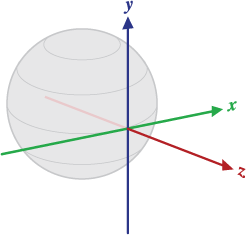
\includegraphics[scale=1]{Gambar/axis-globe.png}
	\caption{Sistem koordinat sensor rotasi vektor terhadap Bumi} 
	\label{fig:axis-globe}
	\end{figure}
	\item values[0]: \(x \sin (\frac{\theta}{2})\)
	\item values[1]: \(y \sin (\frac{\theta}{2})\)
	\item values[2]: \(z \sin (\frac{\theta}{2})\)
	\item values[3]: \(\cos (\frac{\theta}{2})\)
	\item values[4]: Perkiraan akurasi (dalam radians) (-1 jika tidak tersedia) 
\end{itemize}
\section{Google VR SDK}
\label{sec:google_vr_sdk}
Google VR SDK\cite{google_vr_developers} digunakan untuk membantu dalam pembuatan aplikasi Virtual Reality pada \textit{smartphone}. Google VR SDK memberikan beberapa fitur sebagai berikut :
\begin{itemize}
	\item \textbf{Binocular rendering}: Fitur untuk tampilan layar terpisah untuk masing-masing dalam pandangan VR.
	\item \textbf{Spatial audio}: Fitur untuk mengeluarkan suara yang datang dari daerah-daerah tertentu dari dunia VR.
	\item \textbf{Head movement tracking}: Fitur untuk mendapatkan memperbaharui pengelihatan dunia VR yang sesuai dengan gerakan kepala pengguna.
	\item \textbf{Trigger input}: Fitur untuk memberikan input pada dunia VR dengan menekan tombol.
\end{itemize}

Ada beberapa persyaratan untuk menggunakan Google VR SDK, persyaratan tersebut adalah:
\begin{itemize}
	\item Android Studio versi 1.0 atau lebih.
	\item Android SDK versi 23
	\item Gradle versi 23.0.1 atau lebih. Android Studio akan membantu meningkatkan versinya jika versinya terlalu rendah.
	\item Perangkat Android fisik yang menjalankan Android versi 4.4 (KitKat) atau lebih.
\end{itemize}

Dalam membuat aplikasi Google Cardboard VR membutuhkan beberapa API(Application Program Interface) dari Google VR SDK. API-API umum yang akan digunakan adalah sebagai berikut. 
\begin{itemize}
	\item API audio: API untuk mengimplementasikan \textbf{\textit{Spatial Audio}} (Metode untuk menspasialisasikan sumber suara dalam ruang tiga dimensi).
	\item API base: API untuk fondasi dari suatu aplikasi Google VR.
\end{itemize}

\subsection{API Audio}
\label{sec:api_audio}
API ini membantu developer untuk menspasialisasikan sumber suara dalam tiga dimensi, termasuk jarak dengan tinggi isyarat sumber suara. Pada API ini hanya terdapat satu class utama yaitu \textbf{GvrAudioEngine}. \textbf{GvrAudioEngine} mampu memutarkan suara secara spasial dalam dua cara yang berbeda :
\begin{itemize}
	\item Metode pertama dikenal sebagai \textit{Sound Object rendering}. Metode ini memungkinkan pengguna membuat sumber suara virtual dalam ruang tiga dimensi.
	\item Metode kedua memungkinkan pengguna untuk memutar kembali rekaman \textit{Ambisonic soundfield}. Rekaman \textit{Ambisonic soundfield} adalah file audio \textit{multi-channel} yang telah terspasialisasi.
\end{itemize}
API ini juga dapat memutarkan suara secara \textit{stereo}. Kelas \textbf{GvrAudioEngine} memiliki tiga buah \textit{nested class} yaitu:
\begin{itemize}
	\item GvrAudioEngine.DistanceRolloffModel: Kelas ini mendefinisikan konstanta-konstanta yang merepresentasikan perbedaan jarak dari efek model-model rolloff. 
	\item GvrAudioEngine.MaterialName: Kelas ini mendefinisikan konstanta-konstanta yang merepresentasikan bahan permukaan ruangan untuk disesuaikan dengan efek suara pada suatu ruangan.
	\item GvrAudioEngine.RenderingMode: Kelas ini mendefinisikan konstanta-konstanta untuk menyesuaikan dengan mode rendering. Semakin baik kualitas renderin akan semakin besar penggunaan CPU(Central Processing Unit).
\end{itemize}

\subsection{API Base}
\label{sec:api_base}
API ini digunakan sebagai fondasi dari suatu aplikasi Google VR. Fitur-fitur Binocular rendering, Head movement tracking, dan Trigger input diimplementasikan pada API ini. Kelas-kelas penting yang ada di API ini adalah AndroidCompat, Eye, GvrActivity, GvrView, HeadTransform, Viewport.
\begin{itemize}
	\item AndroidCompat\\
Kelas ini merupakan kelas utilitas untuk menggunakan fitur VR. Fitur-fitur ini mungkin tidak tersedia pada semua versi android. Kelas ini memiliki method-method sebagai berikut:
\begin{itemize}
	\item setSustainedPerformanceMode(Activity activity, boolean enabled): \\
	Method ini digunakan untuk mengubah window android ke mode performa secara berkelanjutan.
	\item public static void setVrModeEnabled (Activity activity, boolean enabled): \\
	Mengatur pengaturan yang tepat untuk "mode VR" pada suatu Activity. Method ini tidak digunakan karena hanya dapat digunakan pada Android N+.
	\item public static boolean trySetVrModeEnabled (Activity activity, boolean enabled): 
	Method ini kegunaanya sama dengan method \textbf{setVrModeEnabled (Activity activity, boolean enabled)}, namun mengembalikan boolean true jika berhasil dan sebaliknya.
\end{itemize}
	\item Eye\\
Kelas ini mendefinisikan detil perenderan stereoskopik mata. Method penting yang dimiliki kelas ini adalah \textbf{public float[] getEyeView ()}. Method ini mengembalikan matriks yang mentransformasikan camera virtual ke mata. Transformasi yang diberikan termasuk melacak rotasi kepala, perubahan posisi dan perubahan IPD(interpupillary distance).
	\item GvrActivity\\
Kelas ini merupakan Activity dasar yang menyediakan integrasi yang mudah dengan headset Google VR. Kelas ini mengekspos kejadian untuk berinteraksi dengan headset Google VR dan menangani detil-detil yang biasa diperlukan saat membuat suatu Activity untuk perenderan VR. Activity ini membuat layar tetap menyala selama perangkat android bergerak. Jika tidak ada pergerakan dari perangkat android maka layar reguler (\textit{wakeclock}) akan ditampilkan. Pada kelas ini terdapat method \textbf{onCardboardTrigger ()} untuk mendeteksi ketika Cardboard Trigger sedang ditarik dan dilepaskan (Magnet yang berada pada sisi Google Cardboard).
	\item GvrView\\
	Kelas ini merupakan kelas View yang menyediakan perenderan VR. Kelas ini didesain untuk berkerja pada mode layar penuh dengan orientasi \textit{landscape} atau \textit{reverse landscape}. Kelas View ini dapat digunakan dengan mengimplements salah satu Interface perenderan. Interface-interface tersebut adalah:
	\begin{itemize}
		\item GvrView.StereoRenderer: Interface untuk perenderan detil stereoskopik secara abstrak oleh perender.
		\item GvrView.Renderer: Interface untuk mesin yang kompleks yang membutuhkan untuk menangai semua detil perenderan.
	\end{itemize}
Kelas GvrView.Renderer jarang digunakan dan sebaiknya tidak digunakan jika tidak sangat dibutuhkan.
Ketika suatu kelas mengimplement Kelas GvrView.StereoRenderer, kelas tersebut harus mengimplementasikan method-method berikut ini:
\begin{itemize}
	\item \textbf{public void onNewFrame(HeadTransform headTransform)}\\
	method ini terpanggil ketika Framebaru akan digambar. Method ini memungkinkan untuk membedakan antara perenderan pandangan mata dan frame-frame yang berbeda. Setiap operasi per-frame harus tidak spesifik pada satu tampilan saja.
	\item \textbf{public abstract void onDrawEye (Eye eye)}\\
	Method ini meminta untuk menggambar suatu konten dari sudut pandang mata.
	\item \textbf{public abstract void onFinishFrame (Viewport viewport)}\\
	Method ini dipanggil ketika suatu frame telah selesai. Dengan pemanggilan ini, konten frame telah di gambar dan jika koreksi distorsi diaktifkan, koreksi distrosi akan diterapkan. Setiap perendereran pada tahap ini relatif terhadap seluruh permukana, tidak terhadap satu pandangan mata tunggal. 
	\item \textbf{public abstract void onRendererShutdown ()}\\
	Method ini dipanggil ketika thread perender sedang menutup. Melepaskan sumber GL(Graphics Library) dan sedang melakukan penutupan operasi pada thread perender. Dipanggil hanya jika sebelumnya ada pemanggilan method onSurfaceCreated.
	\item \textbf{public abstract void onSurfaceChanged (int width, int height)}\\
	Dipanggil ketika ada perubahan dimensi permukaan. Semua nilai adalah relatif ke ukuran yang dibutuhkan untuk merender sebuah mata.
	\item \textbf{public abstract void onSurfaceCreated (EGLConfig config)}\\
	Method ini dipanggil ketika suatu permukaan dibangun atau dibangun ulang.
\end{itemize}
\item HeadTransform\\
	Method ini mendeskripsikan transformasi kepala secara independen dari setiap parameter mata. Kelas ini digunakan di kelas GvrView.StereoRenderer sebagai parameter pada method \textbf{onNewFrame}. Method-method yang perlu diperhatikan pada kelas ini adalah:
	\begin{itemize}
		\item \textbf{public void getHeadView (float[] headView, int offset)}\\
		Method ini digunakan untuk mendapatkan matriks transformasi dari camera virtual ke kepala. Kepala disini didefinisikan sebagai titik tengah diantara kedua mata. Matriks yang didapatkan akan disimpan pada parameter \textbf{headView}.
		\item \textbf{public void getQuaternion (float[] quaternion, int offset)}\\
		Method ini digunakan untuk mendapatkan quaternion yang merepresentasikan rotasi kepala.
	\end{itemize}
	\item Viewport\\
	Kelas ini didefinisikan sebagai \textit{viewport}(area pandang) berbentuk persegi.
\end{itemize}
\section{Head Motion Detection Menggunakan Camera Inframerah}
\label{sec:head_motion_detection}
\cite{kapoor2001real}Mengangguk kepala dan menggeleng kepala merupakan gerakan non-verbal yang sering digunakan untuk berkomunikasi.  Arah dari pergerakan kepala dapat diperoleh dari posisi pupil pada camera. Posisi pupil pada camera ini digunakan pada observasi diskrit Hidden Markov Model(HMM) berdasarkan pola alat analisa untuk mendeteksi kepala ketika sedang mengangguk atau menggeleng. Sistem ini akan dilatih dan diuji pada data rekaman dari sepuluh pengguna dengan variasi pencahayaan dan ekspresi muka. Sistem ini memiliki tingkat akurasi sebesar 78.46\% berdasarkan pada data tes.
\subsection{Probabilitas Kemungkinan dan Kebebasan}
Terkadang kita memiliki pengetahuan tentang hasil dari suatu eksperimen dan secara alamiah mungkin mempengaruhi hasil pencobaan lainnya. Pengetahuan ini dapat di peroled dengan konsep probabilitas bersyarat. Kemungkinan dari suatu kejadian sebelum mempertimbahkan pengetahuan tambahan disebut juga \textit{prior probability} dari suatu kejadian. Kemungkinan dari hasil penggunaan pengetahuan tambahan disebut dengan \textit{posterior probability} dari suatu kejadian. Probabilitas bersyarat dari suatu kejadian A yang terjadi setelah kejadian B terjadi(\(P(A|B)\)) dengan Peluang B lebih besar dari 0 (\(P(B)>0\)) adalah:
\begin{align*}
	P(A|B) =& \frac{P(A\cap B)}{P(B)}\\
	&atau,\\
	P(A|B) =& \frac{P(A,B)}{P(B)}
\end{align*}
bahkan jika P(B) = 0, masih dapat diselesaikan dengan aturan perkalian:
\[
	P(A\cap B) = P(B)P(A|B) = P(A)P(B|A)
\]
Generalisasi dari aturan ini untuk banyak kejadian adalah sebagai berikut, atau disebut juga sebagai \textit{chain rule}:
\[
	P(A_1\cap ...\cap A_n)=P(A_1)P(A_2|A_1)P(A_3|A_1\cap A_2)...P(A_n|\cap^{n-1}_{i=1} A_i)
\]
\textit{Chain rule} ini akan digunakan dalam Markov Model.
Kejadian A dengan B bersifat independen. Hal ini menyebabkan jika \(P(A\cap B) = P(A)P(B)\) kecuali \(P(B) = 0 \) akan menghasilkan persamaan \(P(A) = P(A|B)\)
\subsection{Markov Model} 
\label{sec:markov-model}
\cite{manning1999natural} 
\begin{figure}[htbp]
	\centering
		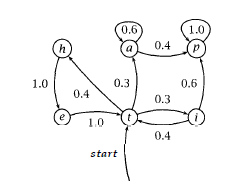
\includegraphics{Gambar/markov-model-example.png}
	\caption{Contoh Markov Model}
	\label{fig:markov-model-example}
\end{figure}
Markov model dapat digunakan ketika ingin memodelkan probabilitas dari suatu urutan linear pada suatu peristiwa. Contohnya, markov model yang digunakan dalam pemodelan urutan tutur perkataan dalam suatu dialog. Selain itu markov model juga digunakan untuk pengenal suara dan lain-lain. 
Deret Markov menggunakan 
Deret Markov dapat merepresentasikan oleh Markov model dengan suatu State Diagram seperti pada gambar \ref{fig:markov-model-example}. Transisi yang mungkin terjadi digambarkan dengan panah yang menghubungkan antar kondisi, dan pada lengkungan panahnya di berikan label probabilitas dari transisi tersebut. Jumlah dari seluruh probabilitas yang keluar dari suatu kondisi akan berjumlah 1. Dalam Markov Model, dapat diketahui bahwa kondisi-kondisi yang akan suatu mesin tempuh, sehingga urutan kondisi atau beberapa fungsi deterministik dapat dijadikan sebagai pengeluaran. 
Probabilitas dari suatu urutan kondisi (yaitu urutan dari variabel-variabel random) \(X_i,...,X_T\) dapat dengan mudah di kalkukasi dengan deret Markov. Deret Markov dapat direpresentasikan dengan persamaan berikut:
\begin{align*}
P(X_1,...,X_T) =& P(X_1)P(X_2|X_1)P(X_3|X_1,X_2)...P(X_T|X_1,...,X_{T-1})\\
=& P(X_1)P(X_2|X_1)P(X_3|X_2)...P(X_T|X_1,...,X_{T-1})\\
=& \pi_{X_1} \Pi^{T-1}_{t=1} A X_t X_{t+1}
\end{align*}\\
Jadi, dengan Markov Model pada gambar \ref{fig:markov-model-example}, didapatkan:
\begin{align*}
	P(t,i,p) =& P(X_1 = t)P(X_2 = i|X_1 = t)P(X_3 = p|X_2 = i)\\
	 =& 1.0 \times* 0.3 \times* 0.6\\
	 =& 0.18
\end{align*}

\subsubsection{Hidden Markov Models}
\label{sec:hidden-markov-models}
Pada HMM(Hidden Markov Models), tidak dapat diketahui urutan kondisi yand dilewati model, tetapi hanya beberapa fungsi probabilistik saja yang diketahui. HMM berguna ketika dapat memikirkan peristiwa secara probabilistik yang menghasilkan peristiwa muka. 

\textbf{Bentuk Umum HMM}\\
HMM dispesifikasikan dengan (\(S,K,II,A,B)\), dimana S dengan K adalah kumpulan kondisi dan keluaran alphabet, dan II, A, dan B adalah probabilitas untuk kondisi awal, kondisi transisi, dan emisi simbul, secara berturut-turut. Notasi-notasi tersebut akan dijelaskan lebih lanjut pada tabel \ref{tab:hmm-notation}

\begin{table}%
	\centering
\begin{tabular}{l l}
Kumpulan kondisi  & \(S=\{ s_1,...,s_N\}\)\\
Keluaran alphabet	& \(\{k_1,...,k_M\} = \{1,...,M\}\)\\
\\
Probabilitas kondisi awal & \(II = \{\pi_i\}, i\in S\)\\
Probabilitas kondisi transisi & \(\{a_{ij}\},i,j\in S\)\\
Probabilitas emisi simbol & \(\{a_{ij}\},i,j\in S\)\\
\\
Deretan kondisi	& \(x= (X_,...,X_{T+1}) X_t : s \stackrel{}{\rightarrow} \{1,...,M\}\)\\
Deretan keluaran & \(O= (o_1,...,o_T) O_t \in K\)
\end{tabular}
\caption{Notasi yang digunakan dalam HMM}
\label{tab:hmm-notation}
\end{table}


\textbf{Mencari Probabilitas dari Suatu Observasi}
Diberikan suatu urutan observasi \(O = (o_1,...,o_T)\) dan suatu model \(\mu = (A,B,II)\), yang ingin dicari adalah bagaimana mengkalukasi \(P(O|\mu )\) secara efisien. Proses ini sering disebut juga sebagai \textit{decoding}. Untuk semua deret kondisi \(X = (X_1,...,X_{T+1})\),
\begin{align*}
	P(O|X,\mu ) =& \Pi^{T}_{t=1} P(o_t|X_t,X_t+1,\mu )\\
		=& b_{X_1 X_2 o_1}b_{X_2 X_3 o_2}... b_{X_T X_{T+1}o_T}
\end{align*}
dan, 
\[
	P(X|\mu ) = \Pi_{X_1}a_{X_1 X_2}a_{X_2 X_3}...a_{X_T X_{T+1}}\\
\]
adapun,
\[
	P(O,X|\mu ) = P(O|X,\mu ) P(X|\mu )
\]
olehkarena itu, 
\begin{align*}
	P(O|\mu ) =& \Sigma_X P(O|X,\mu ) P(X|\mu )\\
	=& \Sigma_{X_1 ...X_{T+1}} \pi X_1 \Pi^{T}_{t=1} a_{X_t X_{T+1}}b_{X_t X_{t+1}o_T}
\end{align*}
Penurunan ini cukup terang-terangan. Sayangnya, evaluasi langsung dari ekspresi yang dihasilkan tersebut sangatlah tidak efisien. Untuk kasus umum (kasus yang dapat dimulai pada kondisi apapun, dan pindah ke kondisi lain pada setiap tahapnya), kalkukasinya membutuhkan \((2T+1).T^{T+1}\) Untuk menangai kompleksitas ini dapat menggunakan teknik umum yaitu \textit{dynamic programming memoization} yang mengingat sebagian hasil dibandingkan harus menghitung ulang kembali. Untuk algoritma seperti HMM, \textit{dynamic programming} secara umum dideskripsikan dalam bentuk dari \textit{trellises}(bisa juga disebut dengan \textit{laticces}). \textit{Trellis} dapa merekan probabilitas semua \textit{subpaths} awal dari suatu HMM yang berakhir pada kondisi tertentu pada waktu tertentu. Probabilitas dari \textit{subpaths} yang lebih panjang dapat digunakan untuk suatu hal dari \textit{subpaths} yang lebih pendek.
\section{Teori Quaternion}
\label{sec:teori_quaternion}
Pada Android SDK \textbf{SensorEvent.values} \cite{android_developers} tipe sensor \textbf{Sensor.TYPE\_ROTATION\_VECTOR}, yaitu tipe sensor yang mendeteksi vektor perputaran pada \textit{smartphone}. Tipe sensor ini dijelaskan akan mengembalikan nilai-nilai dari komponen quaternion. 
Quaternion\cite{kuipers:1999} adalah objek penggabungan dari suatu skalar dengan suatu vektor, sesuatu yang tidak dapat didefinisikan dalam aljabar linear biasa. 

\subsection{Struktur Ajabar}
Struktur-Struktur aljabar yang digunakan adalah Bilangan Kompleks, Konjugasi Kompleks, \textit{Quaternion Algebra}, dan Operasi-operasi pada \textit{Quaternion}.

\subsubsection{Bilangan Kompleks}

Dalam matematika, bilangan kompleks adalah bilangan yang berbentuk\\
\[
	a+bi
\]\cite{kuipers:1999}\\
dan \(a\) dengan \(b\) merupakan bilangan riil, dan \(i\) merupakan bilangan imajiner tertentu yang memiliki sifat \(i^2=-1\).

Berikut notasi-notasi bilangan kompleks :
\[
 (a + bi) + (c + di) = (a+c) + i(b+d)
\]
\[
 (a + bi)(c + di) = (ac−bd) + (bc+ad)i
\]
\[
 a(c + id) = ac + iad
\]
Bilangan kompleks dapat digunakan untuk rotasi dua dimensi. Dengan \(a = \cos (\frac{\theta}{2})\), dan \(b = \sin(\frac{\theta}{2})\), kemudian akan dikalikan dengan vektor yang ingin di putar, dengan sumbu putar adalah titik pusat.


\subsubsection{Konjugasi Kompleks}
\cite{kuipers:1999}Berhubungan dengan bentuk umum bilangan kompleks,
\[
	z = a + ib
\]\\
satu bilangan dikatakan konjugasi kompleks jika
\[
	\bar{z} = a - ib
\]\\
Dari kedua persamaan diatas dapat dihasilkan :
\[
	z + \bar{z} = 2a
\]dan,
\[
	z \bar(z) = a^2 +b^2 = |z|^2
\]

\subsection{\textit{Quaternion Algebra} dan Operasi-operasi pada Quaternion}
\cite{kuipers:1999}Pada buku "Quaternions and Rotation Sequences : A Primer with Applications to Orbits, Aerospace, and Virtual Reality" disebutkan :
\begin{quote}
In 1843 Hamilton invented the so-called hyper-complex number of rank 4, to which he gave the name \textit{quaternion}. Crucial to this invention was his celebrated rule
\[
	i^2 = j^2 = k^2 = ijk = -1
\]
for dealing with the operations on the vector part of the quaternion .
\end{quote}\cite{kuipers:1999}\\
Dari kutipan diatas bilangan \textit{hyper-complex} tingkat empat yang dapat disebut juga \textit{quaternion} memiliki satu aturan yang dicetuskan oleh Hamilton yaitu:
\[
	i^2 = j^2 = k^2 = ijk = -1
\]
Untuk hasil dari perkalian dua \textit{quaternion} memiliki aturan yang lebih rumit, sehingga memiliki aturan-aturan khusus. Berikut aturan-aturan khususnya :
\begin{equation}
	\begin{split}
	& ij = k = -ji\\
	& jk = i = -kj\\
	& ki = j = -ik	
	\end{split}
\label{eq:persamaan_khusus_aturan_quaternion}
\end{equation}\\
Perhatikan bahwa ketiga persamaan diatas mirip dengan cross product vektor sesuai dengan aturan tangan kanan (\textit{right-hand rule}). Dapat di katakan pada Gambar \ref{fig:right-hand-rule}, \(A\) berperan sebagai \(i\), \(B\) berperan sebagai \(j\), dan \(C\) berperan sebagai \(k\). Sehingga terpenuhi sesuai dengan persaman-persamaan \ref{eq:persamaan_khusus_aturan_quaternion}\\
\begin{figure}[htbp]
\centering
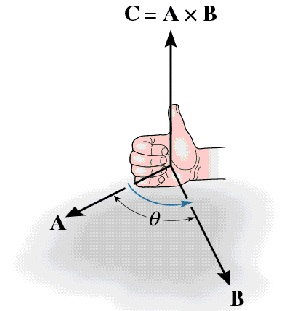
\includegraphics[scale=1]{Gambar/right-hand-rule}
\caption{Right-hand rule dalam \textit{cross product} vektor} 
\label{fig:right-hand-rule}
\end{figure}\\
\textit{Quaternion} memiliki persamaan umum yang memiliki empat bilangan riil atau skalar. Persamaan tersebut adalah 
\[
	q = q_0 + i q_1 + j q_2 + k q_3
\]\cite{kuipers:1999}
Sama seperti pada bilangan kompleks, \textit{quaternion} juga memiliki konjugasi kompleksnya. Berikut adalah konjugasi kompleks \textit{quaternion}
\[
	q = q_0 - i q_1 - j q_2 - k q_3
\]